%!TEX root = <../index.tex>
\section{State of Art}
\label{sec:2}

In this chapter the common methods to calculate similarity between documents are summarized. The methods are usually categorized into two major classes, which are corpus-based and knowledge-based measures. Corpus-based measures try to calculate the value of similarity between documents using information exclusively extracted from large corpora. Normally, the corpora is used both for generating necessary knowledge (e.g. word2vec) and as input data for training models. Meanwhile, the knowledge derived from other resource, e.g. Wikipedia, New York Times, is drawn into the initializing of building models in knowledge-based measures. In our case, the corpus-based measures is preferred rather than knowledge-based measures. The reasons are briefly explained as follows. Firstly, the existent knowledge-based measures are more suitable in the field of word similarity, e.g. \cite{jiang1997semantic}, \cite{strube2006wikirelate} and \cite{Agirre2009ta}, but they are relatively weak for dealing with documents or paragraphs. The second viewpoint is that the prior knowledge has less relevance to the target corpus. The importance and meaning of a word or phrase could be different in difference resource, so that the knowledge from other resource could not interpret identical words in a specific corpus.  Furthermore, the knowledge-based measures have relatively unsatisfactory performance in case of dealing with the considerable number of Out of Vocabulary (OOV) words, whereas exactly compound words and inflection are ubiquitous in German.

In the following subsection, the traditional approaches of semantic text similarity are introduced. After that, a few of important measures of Vector Space Model (VSM) are described. The third part focuses on a short review of existent recommendation systems. The section concludes with a formulation of the research questions. 

\subsection{Traditional STS Methods}
\label{sec:2.1}

\cite{bar2013composite} proposes a classification schema which categorizes the measures into \textit{compositional measures} and \textit{non-compositional measures}. In short, \textit{compositional measures} treat documents as a sequence of words and compute document similarity by aggregating pairwise word similarity.  \textit{Non-compositional measures} regard a document as an entirety and represent it using a model. The overall document similarity is computed by comparing the representations. One of \textit{compositional measures}, introduced in \cite{islam2008semantic} and three \textit{non-compositional measures}, called LCS, GTS, Jaccard Coefficient respectively, are described as follows.

\subsubsection{Longest Common Substring/Subsequence}

Longest common substring is based on a basic idea that document is treated as sequence of characters and are compared to each other. The similarity between two texts $t_1$ and $t_2$ is:

\begin{equation}
    sim_{LCS}(t_1, t_2) = 1 -  \frac{l(t_1) + l(t_2) - 2 \cdot l(lcs(t_1, t_2))}{l(t_1) + l(t_2)}
\end{equation}

where the length $l$ of the longest contiguous character sequence $lcs$ is shared between the two texts. Moreover, longest common subsequence overcomes the limitation of continuousness. 

The kind of measures have the drawbacks. One of them is that the measures do not utilize any semantic process, while the measures cannot use any optimization method, so that the operating efficiency is in a low level. Assumed there are $d$ documents in the corpora, average $\overline{w}$ words for each document, and average $\overline{c}$ characters for each word, the time complexity of lcs is $O((d \cdot \overline{w} \cdot \overline{c})^2)$. These drawback occur also in GST, which is drawn in next part. 

\subsubsection{Greedy String Tiling}

Greedy string tiling is implemented by \cite{wise1993string}. The purpose is to detect plagiarism in programming assignment of students. The algorithm works by searching for matches of a maximum-length marking them and continuing the search ignoring marked tokens. Therefore, this method is relatively insensitive the order of words. It makes more sense for similarity computing than LCS. However, the time complexity is worse than LCS. It will be  $O(d^2 \cdot (\overline{w} \cdot \overline{c})^3)$ in the worst case. Taking into consideration of a reasonable efficiency, this method is not used in our experiments.


\subsubsection{\cite{islam2008semantic}}

\cite{islam2008semantic} introduces an extension of longest common subsequence, that computes not only the scores of lcs ($v_1$), but also the scores of maximal consecutive longest common subsequence at character 1 ($v_2$) and at character n ($v_3$). The overall score of similarity is the weighted mean of the three scores, mathematically, $sim = w_1v_1 + w_2v_2 + w_3v_3$, where $w_1 + w_2 + w_3 = 1$. 

The above described three measures regard documents as sequences of characters, so that they are not able to represent the latent relatedness of documents and they are no longer in force when they deal with long (and with multiple semantics) documents. Moreover, considering the operating efficiency these measures make sense only for short information such as title and summary of documents. 


\subsubsection{N-gram Models and Jaccard Similarity Coefficient}

From the viewpoint of n-gram models, the elementary unit of documents is not isolated words but combinations of $n$ words, where n equals 2 or 3 typically. N-gram models provide a basic processing idea, that most measures can utilize n-gram models as a part of the workflow, in order to obtain the (probabilistic) association between a word and $n-1$ words as predecessor thereof. One simple and intuitionistic measure is Jaccard similarity coefficient \cite{bank2008calculating}. For two documents $t_1=\{w^1_1, w^2_1, \cdots, w^{|t_1|-n+1}_1\}$, $t_2=\{w^1_2, w^2_2, \cdots, w^{|t_2|-n+1}_2\}$, Jaccard similarity coefficient is defined as the size of the intersection divided by the size of the union. Formally,

\begin{equation}
    sim_{jaccard}(t_1, t_2) = \frac{|t_1 \cap t_2|}{|t_1 \cup t_2|} = \frac{|t_1 \cap t_2|}{|t_1| + |t_2| - |t_1 \cap t_2|}. 
\end{equation}


\subsection{Vector Space Model}
\label{sec:2.2}

The idea of VSMs is to represent a document composed of a word sequence of an uncertain or infinite (e.g. data stream) length as a point in a vector space of a finite and determinate high-dimension. Computing the similarity of two documents $t_1$, $t_2$, is accordingly transformed as computing the similarity of the corresponding vectors $\mathbf{v_1}=(v_1^1, \cdots, v_1^s)$, $\mathbf{v_2}=(v_2^1, \cdots, v_2^s)$. The most common method is to compute $cosine$ similarity:

\begin{equation}
    sim_{cos}(t_1, t_2) = \frac{\mathbf{v_1} \cdot \mathbf{v_2}}{|\mathbf{v_1}| \cdot |\mathbf{v_2}|} = \frac{\sum_{i=1}^s v_1^i \cdot v_2^i}{\sqrt{\sum_{i=1}^s (v_1^i)^2} \cdot \sqrt{\sum_{i=1}^s (v_2^i)^2}}
\end{equation}

The $cosine$ similarity of two documents ranges from 0 to 1, when all components thereof are non-negative, e.g. in the tf-idf model, while it will rang also from -1 to 1 without the above non-negative requirement, e.g. in topic models. A variant $cosine$ similarity is so-called Pearson correlation, where vectors are normalized by subtracting the vector means $\mathbf{\overline{v}}$.  Mathematically, 

\begin{equation}
    sim_{pearson}(t_1, t_2) = \frac{(\mathbf{v_1-\overline{v}}) \cdot (\mathbf{v_2-\overline{v}})}{|\mathbf{v_1-\overline{v}}| \cdot |\mathbf{v_2}-\mathbf{\overline{v}}|}
\end{equation}

Another measure to indicate the similarity of vectors is to compute the distance, such as Euclidean distance and Manhattan distance. In this kind of similarity measure, vector normalization must be taken into account. One typical method is to make the norm of vectors as 1, so that documents of different length are treated in the equality. 

\begin{equation}
    sim_{euclidean}(t_1, t_2) = 1 - \frac{\sqrt{\sum_{i=1}^s (v_1^i-v_2^i)^2}}{\sqrt{\sum_{i=1}^s r^2}} ,
\end{equation}
where $r$ is the value range of components of vectors.

VSMs can be classified as term-weighted models and topic-weighted models according to different methods of representing. In following sections we will introduce two common measures of these two types respectively and discuss their advantages and challenges. 

\subsubsection{Bag-of-Words and \textit{tf-idf} Model}

The bag-of-words (BoW) model is a simplest term-weighted vector space model. The vector of a document is composed of the frequency of occurrence of all words in the vocabulary. The dimension of BoW vector therefore is equal to the size of the vocabulary which is normally generated using the entire corpus. The BoW model has a crucial lack that some words occur in the most documents frequently, such as ``go'', ``buy'', ``play'' in English. After normalization, these words will occupy the dominating position and the weight of other words will be	insignificant. Quite the opposite, words, which occur infrequently in the corpus and relatively repeatedly in a cluster, make more sense in the specific context or topic than the common words. 

From this view point, term-frequency-inverse-document-frequency (\textit{tf-idf}) exhibits the importance to provide the meaning or the characteristic in a specific document but not frequency itself of words. The idea contains of two parts. On one side, the metric \textit{tf} indicates how frequent the current word is in the target document. On the other siede, the metric \textit{idf} exhibits the scarcity of the word in the entire corpus. Given a document $d$ from the corpus $D$ and an arbitrary word $w_i$ in the vocabulary, 

\begin{equation}
    tfidf(w_i, d) = tf(w_i, d) \cdot log_2(\frac{|D|}{df(w_i, D)}), 
\end{equation}
where \textit{tf} is the number of occurrences of $w_i$ in $d$, and \textit{df} is the number of documents containing $w_i$. 

In both of BoW and \textit{tf-idf} models, the representation of documents is sparse vectors, of which in average more than 90\% components are zero,  because the vocabulary size is about 10k\textasciitilde 30k and each document has typically 300\textasciitilde 3k words. Furthermore, ignoring the ordering of words in documents for any measure based on the BoW model will lose information of semantics, e.g. relatedness of words, causal relationship between sentences. The former shortcoming will be overcome in topic-weighted measures reviewed in the next paragraphs. 

\subsubsection{Latent Semantic Indexing}

The fundamental idea of LSI is dimensionality reduction, i.e. that documents represented in a high-dimensional term-weighted space are converted into a lower dimensional space, so-called latent semantic space. Each component of vector in the latent semantic space can be understood as the weight of a specific topic.  \cite{Deerwester1990vi} found an way based on linear algebra, called Singular Value Decomposition (SVD), to realize the conversion of vector spaces. Then, \cite{landauer1998introduction} applied the idea to compute semantic similarity. The measure, that the SVD also can be applied for computing document similarity, is called Latent Semantic Indexing (LSI). 

The standard SVD is $N=U\Sigma V^t$, where $\Sigma$ is a diagonal matrix, $U$ and $V$ are orthogonal matrices, i.e. $U^tU=V^tV=I$. The sketch of the process of SVD for the corpora is depicted in figure~\ref{fig:svd} 

\begin{figure}[!htb]
    \centering
    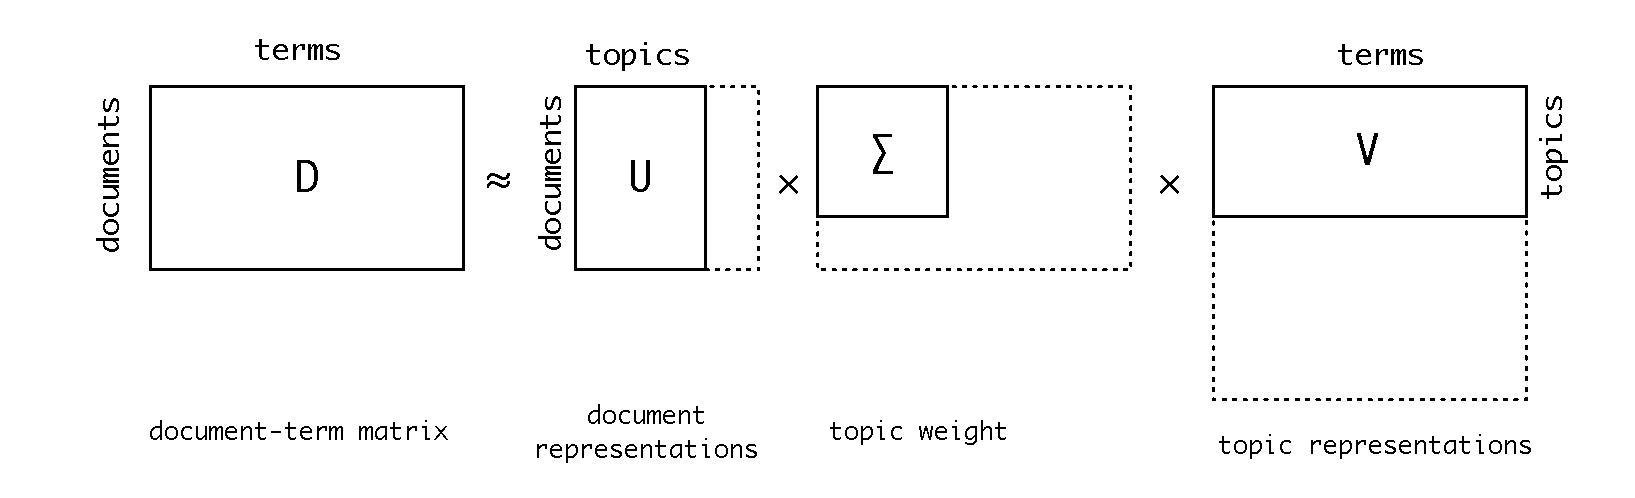
\includegraphics[width=1\textwidth]{fig/SVD.pdf}
    \caption{the sketch of the process of LSI using SVD}
    \label{fig:svd}
\end{figure}

The LSI model is able to recognize synonyms and reduce the adverse impact of noise of data, so that the documents are profiled more precisely and more stably.  However, it has also disadvantages. On the one hand, SVD is an operation with high complexity of runtime and memory. When a huge number of documents are trained or the model needs to update, the cost of SVD is probably intolerable (see section \ref{sec:xxx}). On the other hand, the meaning of the components of $V$ and $U$ cannot be interpreted as a kind of human understanding. 

\subsubsection{Latent Dirichlet Allocation}

LDA was presented as a probabilistic graphical model by \cite{Blei:2003}. LDA is a BoW-based topic model, which can compute the probability distribution of topics for a given document. Moreover, topics can be represented as a series of weighted words by LDA. 

The LDA model (\cite{Blei:2003}) is a Bayesian generative model. From the view point of LDA, a document is generated in the following phases:

\begin{itemize}
    \item[1.] select the topic distribution $\theta_i$ of the target document $d_i$ from the prior Dirichlet distribution $\alpha$, 
    \item[2.] generate a topic $z_{i,j}$ of $j$th word in the document $d_i$ from the multinomial topic distribution $\theta_i$ using Gibbs sampling,
    \item[3.] generate a word distribution $\Phi_{z_{i,j}}$ of the topic $z_{i,j}$ from the prior Dirichlet distribution $\beta$ using Gibbs sampling, 
    \item[4.] generate the word from the multinomial word distribution $\Phi_{z_{i,j}}$. 
\end{itemize}

The progress of generation is illustrated by figure \ref{fig:lda}.

\begin{figure}[!htb]
    \centering
    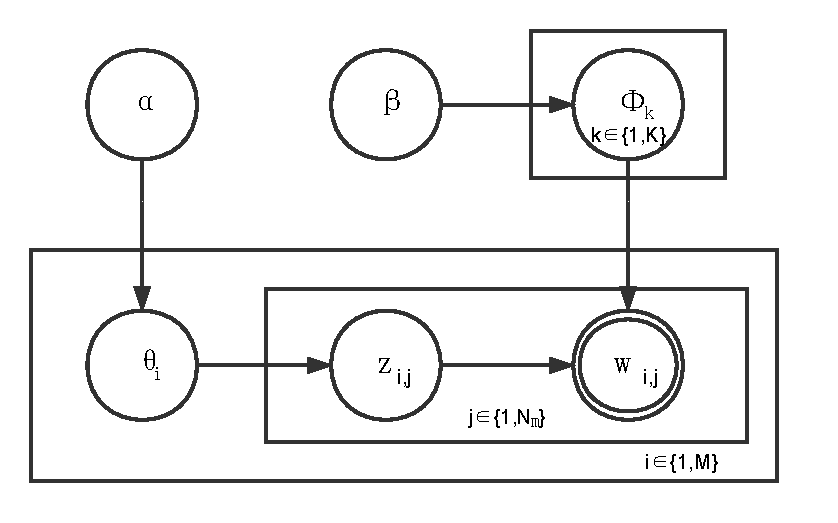
\includegraphics[width=0.5\textwidth]{fig/lda.pdf}
    \caption{Plate notation of representation of LDA. The dual-line plate refers to the observed variable, i.e. the posterior distribution of words in this case, and the monocoil plates indicate the latent variables, such as topic distribution and word distributions given a topic. The direction of arrows refer the conditional dependency of variables. }
    \label{fig:lda}
\end{figure}

The LDA model provides a general idea to build topic model. Since the work of \cite{Blei:2003}, subsequent research has explored many variant of LDA. There are four kinds of topic models so far, where are 1) unsupervised and non-hierarchical, 2) unsupervised and hierarchical, 3) supervised and non-hierarchical and 4) supervised and hierarchical. The research and model names are drawn in the table \ref{tab:lda} respectively.

\begin{table}[!htb]
\centering
\resizebox{\textwidth}{!}{%
\begin{tabular}{|l|l|l|}
\hline
\textbf{Topic Models} & \textbf{non-hierarchical} & \textbf{hierarchical} \\ \hline
\textbf{unsupervised} & \begin{tabular}[c]{@{}l@{}}LDA \cite{Blei:2003} \\ Correlated Topic Model \cite{blei2006correlated} \end{tabular} & HLDA \cite{sivic2008unsupervised} \\ \hline
\textbf{supervised} & \begin{tabular}[c]{@{}l@{}}sLDA \cite{Blei:2008wy} \\ labeled LDA \cite{ramage2009labeled} \end{tabular} & HSLDA \cite{perotte2011hierarchically} \\ \hline
\end{tabular}%
}
\caption{Topic Models Variant of LDA}
\label{tab:lda}
\end{table}

\subsection{Recommendation System}

\subsection{Research Question}

There is a nontrivial way from semantic text similarity to relatedness of documents. We attempt to find a systematic measure to discover related articles by given a target one. The main task is to discover 2\textasciitilde 5 candidate of related articles from a large corpora by given a target document. The most of researches have only discussed the degree of similarity between documents or the proportion of topics in each document and in the corpus. However, text similarity does not mean relatedness, neither do a few shared topics of documents. For example, a piece of news reporting the personal financial problems of the president Obama and another discussing making the financial policy of the president Obama are unrelated to each other by human understanding, whereas the STS measures treat them as related articles due to the high score of text similarity. More about this kind of errors will discuss in section~\ref{}. Four major questions have to be answered, so that achieving the relatedness degree of documents can be formulated more properly: 

\begin{itemize}
    \item[1.] \label{q:1}[1] Can Semantic Text Similarity including string-based and vector space models methods be used to find related articles? How effective and efficient is the metrics of performance, such as precision and operating time?
    \item[2.] \label{q:2}[2] Taking reducing time and memory usage into account, some documents, which are clearly unrelated to the target, should be filtered before processed by STS measures.  Can a filtering method based on data and meta-data be applied to reduce the number candidates that must be checked?
    \item[3.] \label{q:3}[3] Is it useful to combine STS methods with semantic vector space? Does it yield to an improvement in performance or to a significant decrease of runtime?
    \item[4.] \label{q:4}[4] The above introduced methods are unsupervised. Does it lead to an improvement when (semi-) supervised methods are utilized?
\end{itemize}